\documentclass[11pt,a4paper]{article}

% ---------------------------------------------------------------------------
% Repeated selection of inherited chemical states.
%
% Author metadata: set the macros below before submission.  They are
% deliberately blank in this version.  \CompanionAuthor is the author printed
% for the companion manuscripts in refs.bib.
% ---------------------------------------------------------------------------
\newcommand{\PaperAuthor}{}
\newcommand{\PaperAffiliation}{}
\newcommand{\PaperDate}{19 September 2026}
\newcommand{\CompanionAuthor}{Anonymous}
\newcommand{\RepositoryNote}{The repository location will be supplied with the author information.}

\usepackage[T1]{fontenc}
\usepackage[utf8]{inputenc}
\usepackage{lmodern}
\usepackage{microtype}
\usepackage[a4paper,margin=1.05in]{geometry}
\usepackage{amsmath,amssymb,amsthm,mathtools}
\usepackage{booktabs}
\usepackage{array}
\usepackage{enumitem}
\usepackage{xcolor}
\usepackage{graphicx}
\usepackage{tikz}
\usetikzlibrary{arrows.meta,positioning,calc}
\usepackage[obeyspaces,spaces]{url}
\usepackage[numbers,sort&compress]{natbib}
\usepackage[colorlinks=true,linkcolor=blue!55!black,citecolor=blue!55!black,urlcolor=blue!55!black]{hyperref}
\hypersetup{pdftitle={Repeated selection of inherited chemical states: finite-population guarantees and a logarithmic horizon law},
  pdfkeywords={chemical heredity, serial transfer, protocell selection, finite populations, sampling without replacement, Lean}}

\DeclareUrlCommand\lean{\urlstyle{tt}}
\setlist{itemsep=2pt,topsep=3pt}
\setlength{\emergencystretch}{1.5em}
\graphicspath{{figures/}}

\theoremstyle{plain}
\newtheorem{theorem}{Theorem}[section]
\newtheorem{proposition}[theorem]{Proposition}
\newtheorem{lemma}[theorem]{Lemma}
\newtheorem{corollary}[theorem]{Corollary}
\theoremstyle{definition}
\newtheorem{definition}[theorem]{Definition}
\theoremstyle{remark}
\newtheorem{remark}[theorem]{Remark}

\newcommand{\R}{\mathbb R}
\newcommand{\N}{\mathbb N}
\newcommand{\Prob}{\mathbb P}
\newcommand{\E}{\mathbb E}
\newcommand{\eps}{\varepsilon}
\newcommand{\Var}{\operatorname{Var}}
\newcommand{\ind}{\mathbf 1}
\newcommand{\lo}{\mathrm L}
\newcommand{\hi}{\mathrm H}
\newcommand{\fail}{\bot}
\newcommand{\gen}{\mathcal A}

\title{Repeated selection of inherited chemical states:\\[4pt]
\large finite-population guarantees and a logarithmic horizon law}
\author{\PaperAuthor\\ \small \PaperAffiliation}
\date{\PaperDate}

\begin{document}
\maketitle

\begin{abstract}
Serial transfer is the standard way to demonstrate selection in a population of
chemical compartments, but each transfer discards most of the population, and a
state that has become rare can be lost outright to sampling rather than to
chemistry. We prove finite-population guarantees for an arbitrary prescribed
number of such transfers in a fully specified four-species compartment model.
The protocol grows a population on a shared precursor, samples exactly $M$
endpoint compartments uniformly and intact, recovers those same compartments,
and refills in proportion to their actual retained sizes; a finite marked
probability law retains every failure branch and every returned division phase,
and nothing is conditioned on success or resampled. For every horizon $K$ and
every confidence below one there are finite parameters under which both
inherited states remain present at every census while the measured
high-to-low compartment-count log odds exceed $Kg-\log2$, with
$g=\frac35\log4-\frac{19}{500}-\log\frac{51}{49}=0.75377\ldots$. The mission
transfer error is governed by a geometric series whose base is the per-cycle
loss of minority share, and the attainable horizon for this event has order
$\log M$. We then close part of the gap between the sufficient and necessary
constants. A machine-checked exponential-generator inequality is lifted to a
batch statement showing that \emph{both} ancestral size totals grow by a factor
at least $3/2$, which improves the geometric base from $204/49=4.1633$ to
$136/49=2.7755$; a multiplicative concentration bound for weighted uniform
sampling without replacement replaces a Chebyshev tail. Together these move the
sufficient leading coefficient from $1/\log(204/49)=0.7011$ to
$1/\log(136/49)=0.9796$ against a necessary $1/g=1.3267$, and reduce the
population sufficient for a ten-cycle mission from $M=10^{13}$ to
$M=4\times10^{9}$ at higher confidence. Machine-checked statements,
conventional proofs and numerical diagnostics are separated throughout, and
the optimal exponential rate remains open.
\end{abstract}

\tableofcontents

\section{Introduction}\label{sec:intro}

A heritable chemical difference between compartments is selected, in the
laboratory sense, when its share of a population increases across repeated
rounds of growth and dilution~\citep{mills1967,lincoln2009,lenski1991}. For
compartments whose heritable difference is a chemical composition rather than a
template sequence, three separate things must hold for the protocol to work.
The composition must change reproductive output while compartments compete for
a shared resource~\citep{chen2004,adamala2013,lu2024,zwicker2017}; it must be
copied into descendants through growth and the random partition of finitely
many molecules~\citep{segre2000,vasas2010,virgo2015}; and it must survive the
interventions between competitions.

The third requirement is the one that finite population size makes sharp, and
it is the subject of this paper. Every transfer removes most of the population.
Selection makes the disfavoured state rare, and a rare state is lost to the
sampling step for reasons that have nothing to do with its
chemistry~\citep{wahl2001,wahl2002}. Consequently a one-cycle or two-cycle
theorem does not iterate: the cells that begin cycle $j+1$ are the actual cells
retained at the end of cycle $j$, with heterogeneous sizes and division phases,
and the minority share available as an inductive hypothesis has decayed.

\subsection{What is proved}

We work with one fully specified stochastic source: a four-species count
network with thirteen resident channels inside each compartment, a shared
growth precursor, complementary division at doubled size, uniform intact-cell
transfer, a precursor-free recovery interval, and proportional refill
(Section~\ref{sec:model}). The probability space is a finite marked law in
which every failure branch keeps its mass in an absorbing failure symbol
(Section~\ref{sec:law}). The following are the principal statements.

\begin{enumerate}[label=(\roman*)]
\item \emph{A mission guarantee at every finite horizon}
(Theorem~\ref{thm:main}). For every $K$, every even $M$, and admissible
$N,\gamma$ and finite service quotas, the composed source law assigns
probability at least
\[
1-K\,E(N,M,T)-\frac{80000}{M}\sum_{j<K}\Bigl(\frac{204}{49}\Bigr)^{j}-K(s_B+s_R)
\]
to an event on which all $K$ cycles return ready populations, both measured
chemical counts are positive at every census, the ancestry size shares obey
$q_{b,j}\ge\frac12\rho^{j}$ with $\rho=49/204$, and the measured count log odds
satisfy $L_j-L_0>jg-\log2$ for every $j\le K$. For every prescribed $K$ and
every confidence below one, finite parameters achieving it exist.

\item \emph{A logarithmic horizon law} (Corollary~\ref{cor:log} and
Theorem~\ref{thm:order}). The sufficient condition above is an explicit
logarithmic upper bound on $K$, and positivity of two integer counts summing to
$M$ forces $Kg<\log(2(M-1))$. Hence the supremum attainable integer horizon
\emph{for this gain event}, when molecular scale and service allowances may
increase with $M$, is $\Theta(\log M)$.

\item \emph{An improved exponential base} (Theorem~\ref{thm:growth} and
Theorem~\ref{thm:refined}). A machine-checked scalar generator inequality is
lifted to the batch: on the certified event, \emph{each} ancestral size total
is at least $\frac32$ times its value at the start of the batch, except with
probability at most $e^{-19N/500000}$, a term already present in the error.
Since the batch quadruples the total size, the per-cycle share loss improves
from $\frac14\cdot\frac{1-\eps}{1+\eps}$ to $\frac38\cdot\frac{1-\eps}{1+\eps}$,
and the geometric base drops from $R=204/49$ to $R_*=136/49$.

\item \emph{An exponential transfer tail} (Proposition~\ref{prop:chernoff}).
For weighted uniform sampling without replacement the second-moment tail
$1/(\eps^2\mu)$ is replaced by $e^{-\eps^2\mu/2}+e^{-\eps^2\mu/(2+\eps)}$, using
Hoeffding's comparison with sampling \emph{with} replacement. A sharp
finite-population variance identity (Proposition~\ref{prop:fpc}) is also
recorded.

\item \emph{Quantitative consequences} (Section~\ref{sec:design}). The
sufficient leading coefficient improves from $0.701115$ to $0.979591$ against
the necessary $1.326662$. A ten-cycle mission that required $M=10^{13}$
compartments at confidence $0.994$ is closed with $M=4\times10^{9}$ at
confidence $0.997$, and $0.999$ with finer service quotas; the terminal
composition guarantee is unchanged, and at least $36\,862$ minority
compartments remain.

\item \emph{Limits} (Sections~\ref{sec:rarity} and \ref{sec:scope}). An exact
hypergeometric identity for the conditional loss of a rare ancestry, complete
material and duration accounts, and an explicit statement of what the model
does and does not calibrate.
\end{enumerate}

\subsection{Three kinds of evidence}\label{sec:evidencekinds}

We keep three categories apart, and label every nontrivial assertion.

\begin{description}[leftmargin=1.9em,style=nextline]
\item[Machine-checked.] The finite marked laws, the conditional composition
induction, the weighted-mean and share-recurrence inequalities, the closed
geometric sum, the chemical sizing envelope, the necessary count ceiling, the
exact conditional loss law, the material accounts, the ten-cycle witness of
Theorem~\ref{thm:witness}, the terminal composition and integer minority
consequences, and the target gain table are verified in Lean~4
\citep{demoura2021,mathlib2020} against a frozen Mathlib. The scalar generator
inequality behind Theorem~\ref{thm:growth} is also verified.
Appendix~\ref{app:formal} maps each claim to its declaration.
\item[Conventional.] The lifting of the scalar inequality to the batch
population statement (Theorem~\ref{thm:growth}), the exponential transfer tail
(Proposition~\ref{prop:chernoff}), the finite-population variance identity
(Proposition~\ref{prop:fpc}), the refined mission theorem
(Theorem~\ref{thm:refined}) and its witness, the $\Theta(\log M)$ formulation,
and the reading of the finite marked laws as an ongoing population process are
ordinary mathematics, written out here in full.
\item[Numerical.] Decimal expansions, the two figures, the eight-cell
enumeration of Section~\ref{sec:hetero}, the reduced deterministic rate
comparison of Section~\ref{sec:scope}, and the parameter grids of
Appendix~\ref{app:formal} evaluate or probe proved formulas. They establish
nothing and simulate no source trajectory. All rational comparisons printed
below are re-derived by an exact replay script with $2083$ assertions
(Appendix~\ref{app:formal}).
\end{description}

\subsection{Relation to prior work}

Compositional heredity has been analysed since \citet{segre2000} and
\citet{szathmary1987}, with sharp doubts about its
evolvability~\citep{vasas2010,vasas2012}; \citet{nowak2008} study selection in
prelife dynamics; \citet{matsubara2026} give analytical conditions for Darwinian
evolution in compartmentalized autocatalytic networks across several
growth-and-division regimes, including Moran-type populations~\citep{moran1958}.
Experimental RNA networks exhibit trade-offs between reproduction, variation and
compositional persistence~\citep{ameta2021}, and the surrounding programme is
framed by the theory of autocatalytic
sets~\citep{kauffman1986,hordijk2004,blokhuis2020}. The dependence of
experimental evolution on bottleneck size is classical in population
genetics~\citep{wahl2001,wahl2002}, as is the observation that asynchronously
dividing lineages can differ in material without differing in
number~\citep{powell1956}, which is why our conclusion is stated in compartment
counts. The present contribution is orthogonal to these: it is a quantitative
finite-count theorem for one fully specified source, with all failure mass
retained, an unconditional mission confidence, and an explicit separation
between chemical fidelity and loss of representation at a finite transfer. We
make no priority claim on chemically driven compartment competition, on
complementary division, or on the serial-transfer protocol, and we do not claim
a theorem for arbitrary autocatalytic networks. The single-batch and two-cycle
predecessors of the present result are the companion
manuscripts~\citep{batch2026,serial2026}; the resident network is taken
unchanged from~\citep{copying2026} and its materially balanced completion
from~\citep{thermo2026}.

\subsection{What is not claimed}

The resident exchange channels are maintained externally; four resident species
do not constitute a closed thermochemically balanced system, and finite gross
exchange allowances count exchanged molecules rather than modelling autonomous
depletion or free energy~\citep{polettini2014,rao2016}. Growth and division are
effective constitutive rules. The coordinate $m$ is an integer model size with
no calibrated volume or molar interpretation (Section~\ref{sec:units}). The
theorem concerns a controlled protocol with externally imposed transfer,
recovery and refill; autonomous environmental cycling is a different statement.
Nothing here establishes indefinite coexistence, fixation, innovation,
open-ended evolution, laboratory feasibility, or optimality of any constant.
The witness parameters are astronomically large because every certificate is
conservative.

\section{The chemical source and the operating protocol}\label{sec:model}

\subsection{Resident channels}\label{sec:chemistry}

A compartment, called a cell, carries an integer size $m$ together with
internal counts $n=(n_A,n_B,n_Z,n_D)\in\N^4$, and its concentration vector is
$x=n/m$. Write $h=1/m$ and $e=10^{-5}$. The resident channels have jump vectors
and density rates of Table~\ref{tab:channels}; the count propensity of a
channel is $m$ times its density rate, and the falling-factorial terms ensure
that propensities vanish on the boundary of the count lattice.

\begin{table}[tb]
\centering\small
\caption{The literal resident source. The fourth resident species is named $D$;
the scale constant $D_0$ of \eqref{eq:D0} is unrelated to it. Channels
$7$--$10$ and $13$ are maintained exchange channels, part of the declared
source rather than autonomous closed-system chemistry.}
\label{tab:channels}
\begin{tabular}{clll}
\toprule
Channel & Count increment $(A,B,Z,D)$ & Density rate & Reading\\
\midrule
1, 2 & $(-1,1,1,0)$; $(1,-1,-1,0)$ & $x_A$; $x_Bx_Z$ & $A\rightleftharpoons B+Z$\\
3, 4 & $(0,0,-1,1)$; $(0,0,1,-1)$ & $16x_Z$; $x_D$ & $Z\rightleftharpoons D$\\
5, 6 & $(0,0,2,-1)$; $(0,0,-2,1)$ & $x_D$; $2x_Z(x_Z-h)$ & $D\rightleftharpoons 2Z$\\
7, 8 & $(1,0,0,0)$; $(-1,0,0,0)$ & $6$; $x_A$ & $A$ exchange\\
9, 10 & $(0,1,0,0)$; $(0,-1,0,0)$ & $27$; $x_B$ & $B$ exchange\\
11, 12 & $(2,-1,0,0)$; $(-2,1,0,0)$ & $ex_B$; $ex_A(x_A-h)$ & $B\rightleftharpoons 2A$\\
13 & $(0,0,0,-1)$ & $x_D/10000$ & $D$ sink\\
\bottomrule
\end{tabular}
\end{table}

The density-limit drift of these channels has two stationary compositions whose
$Z$ coordinates lie in the certified rational intervals
\begin{equation}\label{eq:roots}
z_\lo\in[0.99579401232,\,0.99579401233],\qquad
z_\hi\in[2.97636724376,\,2.97636724377],
\end{equation}
with the remaining coordinates given by the rational formulas of
Appendix~\ref{app:regions}. Their existence and their local stability estimates
are part of the verified source. The two states differ only in their resident
composition; no fitness parameter is assigned, and the only feature that
influences reproduction is the resident concentration of the growth-linked
species $Z$.

\subsection{Growth, division and one complete cycle}\label{sec:cycle}

Let $Q$ be a shared precursor stock with batch reference $\Omega$. Each cell
grows with propensity $\gamma(Q/\Omega)n_Z$, which vanishes when $Q=0$ or
$n_Z=0$. A growth event consumes one unit of $Q$ and one internal $Z$, and
increases $m$ by one. If the resulting size is $2N$, the same event replaces the
parent by two daughters of size $N$: independently for each resident coordinate
$i$, a count $d_i\sim\operatorname{Binomial}(n_i,1/2)$ goes to one daughter and
$n_i-d_i$ to the other, so the partition weight is $\prod_i\binom{n_i}{d_i}2^{-n_i}$
and the two daughters together preserve the post-growth resident counts. The
daughters are complementary, not independent. The ancestry tag carried through
the analysis enters no propensity, no partition draw and no operation of the
protocol.

A \emph{ready population} consists of exactly $M$ cells with sizes in $[N,2N)$
and compositions in the inner neighbourhoods of Appendix~\ref{app:regions}. One
cycle, illustrated in Figure~\ref{fig:protocol}, consists of:

\begin{enumerate}
\item \emph{Batch.} With total size $W_0$, charge $Q=\Omega=4W_0$ and run until
$Q=W_0$, subject to the deadline $T=8/\gamma$. Conservation then gives endpoint
total size $W^-=4W_0$. A division triggered by the terminal growth event is
processed before transfer.
\item \emph{Transfer.} Choose uniformly one subset of exactly $M$ intact
endpoint cells. Remove the other cells and the residual precursor medium.
\item \emph{Recovery.} Hold the selected cells at $Q=0$ for $5376$ model-time
units. Resident chemistry continues; growth and division cease, so sizes and
ancestral totals are frozen.
\item \emph{Refill.} Supply $Q=\Omega=4W_{\rm ret}$ in proportion to the actual
retained total size. On success this is the next ready population.
\end{enumerate}

We require throughout
\begin{equation}\label{eq:admissible}
N\ge N_0:=1.4\times10^{20},\qquad 0<\gamma\le10^{-11}.
\end{equation}

\begin{figure}[tb]
\centering
\resizebox{\linewidth}{!}{%
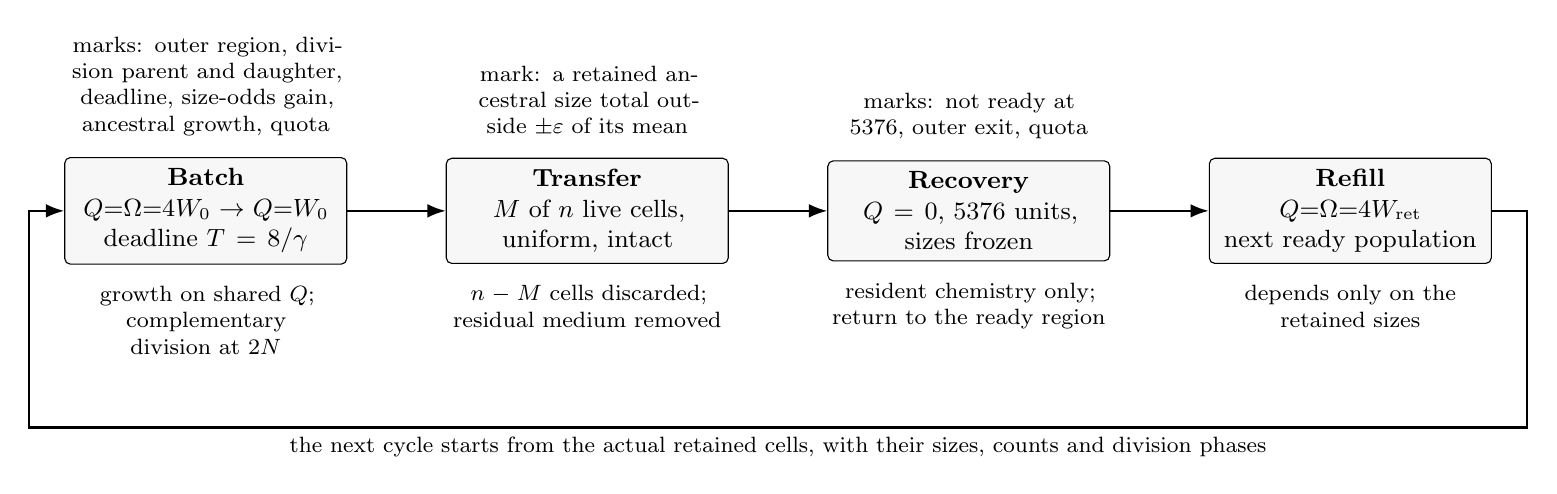
\begin{tikzpicture}[>=Latex,font=\small,
  box/.style={draw,rounded corners=2pt,align=center,minimum height=1.15cm,inner sep=4pt,fill=black!3,text width=3.3cm},
  lab/.style={font=\footnotesize,align=center,text width=3.7cm}]
\node[box] (batch) {\textbf{Batch}\\ $Q{=}\Omega{=}4W_0\to Q{=}W_0$\\ deadline $T=8/\gamma$};
\node[box,right=1.25cm of batch] (transfer) {\textbf{Transfer}\\ $M$ of $n$ live cells,\\ uniform, intact};
\node[box,right=1.25cm of transfer] (recovery) {\textbf{Recovery}\\ $Q=0$, $5376$ units,\\ sizes frozen};
\node[box,right=1.25cm of recovery] (refill) {\textbf{Refill}\\ $Q{=}\Omega{=}4W_{\rm ret}$\\ next ready population};
\draw[->,thick] (batch) -- (transfer);
\draw[->,thick] (transfer) -- (recovery);
\draw[->,thick] (recovery) -- (refill);
\coordinate (br) at ($(refill.east)+(0.45,0)$);
\coordinate (bl) at ($(batch.west)+(-0.45,0)$);
\draw[->,thick] (refill.east) -- (br) -- ($(br)+(0,-2.75)$) -- ($(bl)+(0,-2.75)$) -- (bl) -- (batch.west);
\node[font=\footnotesize,below] at ($(br)!0.5!(bl)+(0,-2.75)$)
  {the next cycle starts from the actual retained cells, with their sizes, counts and division phases};
\node[lab,below=0.15cm of batch] {growth on shared $Q$;\\ complementary division at $2N$};
\node[lab,below=0.15cm of transfer] {$n-M$ cells discarded;\\ residual medium removed};
\node[lab,below=0.15cm of recovery] {resident chemistry only;\\ return to the ready region};
\node[lab,below=0.15cm of refill] {depends only on the\\ retained sizes};
\node[lab,above=0.15cm of batch] {marks: outer region, division parent and daughter, deadline, size-odds gain, ancestral growth, quota};
\node[lab,above=0.15cm of transfer] {mark: a retained ancestral size total outside $\pm\eps$ of its mean};
\node[lab,above=0.15cm of recovery] {marks: not ready at $5376$, outer exit, quota};
\end{tikzpicture}}
\caption{One literal cycle and the analytical marks that define the failure
quotient. Marks enter the analysis only: uniform transfer does not read a
chemical state, and recovery does not reset division phases.}
\label{fig:protocol}
\end{figure}

Because later cycles begin from cells with arbitrary division phases, the
appropriate population cap is $8M$ endpoint cells, not the newborn-only cap
$4M$; every live cell has size at least $N$ and the endpoint total is
$4W_0\le8NM$.

\subsection{Observables}\label{sec:observables}

The chemical readout labels a cell high precisely when $n_Z/m>2$. On ready
states this readout agrees with the ancestry tag, with a wide margin: readiness
forces $\|x-x_*\|_2\le\sqrt{200a}=1/1600$ (Appendix~\ref{app:regions}), so the
largest ready low value of $x_Z$ is at most $0.99641901233$ and the smallest
ready high value is at least $2.97574224376$. Write $C_\hi,C_\lo$ for the
measured counts, $B_\hi,B_\lo$ for the ancestral size totals, $W=B_\hi+B_\lo$,
and
\begin{equation}\label{eq:obs}
q_b=\frac{B_b}{W},\qquad S=\log\frac{B_\hi}{B_\lo},\qquad
L=\log\frac{C_\hi}{C_\lo}.
\end{equation}
Founders are \emph{balanced newborn}: $M$ is even, each state has $M/2$ cells,
and every cell has size exactly $N$; hence $q_{\hi,0}=q_{\lo,0}=\frac12$,
$S_0=0$ and $L_0=0$.

\subsection{The finite marked law}\label{sec:law}

Every stage is a finite marked jump model, uniformized at a finite clock bound
and Poissonized over its duration~\citep{jensen1953,norris1997}, stopped at its
first mark or at its physical endpoint. The output of a stage is either the
actual physical population or a single failure symbol $\fail$, which is
absorbing. Outer-neighbourhood, division, deadline, size-odds, transfer,
recovery and service failures all retain their probability mass in $\fail$.
Stages are composed by binding on returned states, so the law of $K$ cycles is
a probability distribution on histories of ready states or $\fail$. It is never
renormalized on successful trajectories, no failed run is resampled, and no
mark licenses an intervention. The conventional reading of these finite laws as
an ongoing continuous-time population process is the standard
one~\citep{kurtz1972,gillespie1977,andersonkurtz2015}; this paper adds no
identification with an infinite trajectory-space process beyond the existing
source construction.

Let $J_B,J_R$ be positive finite batch and per-cell recovery quotas and let
$q_B,q_R$ be finite uniform clock bounds for the two source models. A counter
that increments on every marked source event and saturates at $J$ leaves the
physical marginal unchanged and saturates by time $t$ with probability at most
$tq/J$. The per-cycle service allowances are therefore
\begin{equation}\label{eq:service}
s_B=\frac{Tq_B}{J_B},\qquad s_R=\frac{M\cdot5376\,q_R}{J_R}.
\end{equation}
Admissible clock bounds exist because the admitted source-state families are
finite; the quotas may then be enlarged to make \eqref{eq:service} as small as
prescribed. This is an existence statement, not an enumeration. Quota capacity
bounds gross event allowances; it is neither actual consumption nor free
energy, and the virtual holds of uniformization are not physical reaction
events.

\subsection{The imported chemical input}\label{sec:input}

Put
\begin{equation}\label{eq:D0}
D_0=5.12\times10^{20},\qquad u=\frac{N}{D_0}=N\alpha a,
\end{equation}
with $\alpha=10^{-12}$ and $a=1/512000000$ the readiness threshold of
Appendix~\ref{app:regions}. The chemical error used throughout is
\begin{align}
E(N,M,T)&=A+e^{-N/2500}+e^{-19N/500000}+M\,R_0(u),\label{eq:E}\\
A&=Me^{-7u}+14Me^{-4u}+\frac{MTu}{42}e^{-15u/2}
 +Me^{-u}+\frac{MTu}{42}e^{-3u/2}\nonumber\\
 &\qquad{}+56Me^{-N/(35\cdot10^{12})},\nonumber\\
R_0(u)&=e^{-u}+2e^{-u/2}+e^{-8u}+16u\,e^{-31u/2}.\nonumber
\end{align}

\begin{proposition}[Source-input proposition; machine-checked]\label{prop:input}
Assume \eqref{eq:admissible}, the stationary roots \eqref{eq:roots}, admissible
finite clocks and positive quotas. Let a batch start from a ready population
with both ancestries present and total size $W_0$. Then, except on an event of
probability at most $E(N,M,T)+s_B+s_R$ under the composed batch-and-recovery
law, the following hold at the batch endpoint and after recovery of the
selected cells.
\begin{enumerate}[label=\emph{(\alph*)}]
\item \emph{Endpoint.} The batch reaches $Q=W_0$ before the deadline $T$; the
endpoint total size is $W^-=4W_0$; every endpoint cell has size in $[N,2N)$ and
lies in the outer region.
\item \emph{Persistence and sandwich.} Both ancestries are present,
$B_b^-\ge B_{b,0}$ for $b\in\{\hi,\lo\}$, and the ancestral $Z$ totals obey
\begin{equation}\label{eq:sandwich}
2.97\,B_\hi\le Z_\hi\le3\,B_\hi,\qquad
0.99\,B_\lo\le Z_\lo\le1.01\,B_\lo
\end{equation}
throughout the batch.
\item \emph{Gain.} The size log odds increase by more than
$b_\star=\frac35\log4-\frac{19}{500}>0.7937$, the shortfall event having
probability at most $e^{-19N/500000}$.
\item \emph{Return.} Each selected cell returns to the ready region after
$5376$ units at $Q=0$, and recovery and refill preserve its size, its tag, and
hence both ancestral size totals and counts.
\end{enumerate}
These conclusions hold for the actual ready input of any cycle, not only for
the initial founders, and the estimates are uniform over admitted inputs.
\end{proposition}

The local exponential chemical barriers, the division concentration bounds
using Hoeffding's inequality~\citep{hoeffding1963}, the size-odds supermartingale
and the recovery estimates behind Proposition~\ref{prop:input} are proved
in~\citep{batch2026,serial2026} and verified; Appendix~\ref{app:formal} lists
the declarations. Part (b) is the ingredient that Section~\ref{sec:refine}
exploits, and \eqref{eq:sandwich} is exactly the certified ancestral rate
window.

\section{The mission theorem}\label{sec:main}

Fix the transfer tolerance $\eps=1/50$ and set
\begin{equation}\label{eq:constants}
\rho=\frac{1-\eps}{4(1+\eps)}=\frac{49}{204},\qquad R=\rho^{-1}=\frac{204}{49},
\qquad g=b_\star-\log\frac{51}{49}=0.7537712820\ldots>\frac34 .
\end{equation}
Let $\mathcal G_K$ be the event that all $K$ cycles return ready populations,
that both measured counts are positive at every census, and that
\begin{equation}\label{eq:gain}
L_j-L_0>jg-\log2,\qquad 1\le j\le K .
\end{equation}

\begin{theorem}[Mission guarantee; machine-checked]\label{thm:main}
Let $K\in\N$, let $M\ge2$ be even, and let $N,\gamma$ satisfy
\eqref{eq:admissible}. Choose the stationary roots \eqref{eq:roots}, admissible
finite clocks, positive quotas, and balanced newborn founders. Under the
original composed source law there is an event
$\mathcal H_K\subseteq\mathcal G_K$ with
\begin{equation}\label{eq:prob}
\Prob(\mathcal H_K)\ \ge\
1-K\,E(N,M,T)-\frac{80000}{M}\sum_{j=0}^{K-1}R^{\,j}-K(s_B+s_R),
\end{equation}
and on $\mathcal H_K$, for both states and every $0\le j\le K$,
\begin{equation}\label{eq:floors}
q_{b,j}\ge\tfrac12\rho^{\,j},\qquad \frac{C_{b,j}}{M}\ge\tfrac14\rho^{\,j}.
\end{equation}
For every prescribed finite $K$ and every $0<\delta<1$, finite parameters and
quotas exist with $\Prob(\mathcal H_K)\ge1-\delta$.
\end{theorem}

The final assertion does not keep $M$ fixed as $K$ grows. Neither does
\eqref{eq:gain} assert monotone improvement between adjacent censuses: it is a
cumulative statement measured from the founders.

\subsection{Weighted shares are the right inductive quantity}\label{sec:shares}

Condition on a complete batch endpoint with $n$ cells of sizes
$m_i\in[N,2N]$. For ancestry $b$ put
\begin{equation}\label{eq:weights}
w_{b,i}=\frac{m_i}{2N}\,\ind_{\{b_i=b\}}\in[0,1],\qquad
X_b=\sum_{i\ \mathrm{selected}}w_{b,i}.
\end{equation}

\begin{lemma}[Mean of a weighted retained total]\label{lem:mean}
Under the uniform law on $M$-subsets,
$\mu_b=\E X_b=\frac{M}{n}\frac{B_b^-}{2N}$. If moreover $nN\le W^-=4W_0$ and
$B_b^-\ge\lambda B_{b,0}$ for some $\lambda\ge1$, then
\begin{equation}\label{eq:meanfloor}
\mu_b\ \ge\ \frac{\lambda}{8}\,M\,q_{b,0}.
\end{equation}
\end{lemma}

\begin{proof}
Each cell is included with probability $M/n$, so
$\mu_b=(M/n)\sum_iw_{b,i}=(M/n)B_b^-/(2N)$. Every live cell has size at least
$N$, so $nN\le W^-$, that is $M/n\ge MN/(4W_0)$. Hence
$\mu_b\ge\frac{MN}{4W_0}\cdot\frac{\lambda B_{b,0}}{2N}
=\frac\lambda8 M\frac{B_{b,0}}{W_0}$.
\end{proof}

With the persistence statement $B_b^-\ge B_{b,0}$ of
Proposition~\ref{prop:input}(b), Lemma~\ref{lem:mean} applies with $\lambda=1$
and gives $\mu_b\ge Mq_{b,0}/8$; Section~\ref{sec:refine} improves $\lambda$.

\begin{lemma}[Variance at most mean]\label{lem:var}
The inclusion indicators of distinct cells have nonpositive covariance, and for
weights in $[0,1]$, $\Var(X_b)\le\mu_b$.
\end{lemma}

\begin{proof}
Permutation symmetry gives $\E I_i=M/n$ and
$\E I_iI_k=M(M-1)/(n(n-1))\le(M/n)^2$ for $i\ne k$, the inequality being
equivalent to $M\le n$. Dropping the nonpositive cross terms,
$\Var(X_b)\le\sum_iw_{b,i}^2\Var(I_i)\le\sum_iw_{b,i}\E I_i=\mu_b$, using
$w^2\le w$ and $\Var(I)\le\E I$ for an indicator.
\end{proof}

Chebyshev's inequality then bounds the one-type relative failure by
$1/(\eps^2\mu_b)$, and a union over the two ancestries, with $\mu_b\ge Mq/8$
when both input shares are at least $q$, bounds the transfer failure by
\begin{equation}\label{eq:transferbound}
\frac{16}{\eps^2Mq}.
\end{equation}
On the complementary event both retained ancestral totals lie within relative
tolerance $\eps$ of their means, which carry the common factor $M/n$; hence
\begin{equation}\label{eq:recurrence}
q_b^+\ \ge\ \frac{1-\eps}{1+\eps}\,q_b^-\ \ge\ \frac{1-\eps}{4(1+\eps)}\,q_b
=\rho\,q_b ,
\end{equation}
using $B_b^-\ge B_{b,0}$ and $W^-=4W_0$ for the second inequality. Recovery and
refill preserve the selected sizes and ancestral totals
(Proposition~\ref{prop:input}(d)), so \eqref{eq:recurrence} is the share of the
next ready population.

\begin{remark}[Why shares and not counts]\label{rem:shares}
At a ready census $B_b\le2NC_b$ and $W\ge NM$, so $C_b/M\ge q_b/2$. This factor
of two is an \emph{endpoint conversion}, applied once when a share statement is
read as a count statement. The earlier count-floor argument paid it inside the
recurrence at every cycle, producing the geometric base $800/49$ and the
mission budget $(160000/M)\sum_{j<K}(800/49)^j$. Propagating size shares and
converting once is the structural improvement behind \eqref{eq:prob}.
\end{remark}

\subsection{Composition over the history}\label{sec:composition}

\begin{proof}[Proof of Theorem~\ref{thm:main}]
Set $q_j=\frac12\rho^{\,j}$. Suppose a realized prefix of $j$ cycles is
successful, so that both input shares of cycle $j$ are at least $q_j$. By
Proposition~\ref{prop:input} and \eqref{eq:transferbound}, the conditional
probability that cycle $j$ fails is at most
\begin{equation}\label{eq:dj}
d_j=E(N,M,T)+\frac{16}{\eps^2Mq_j}+s_B+s_R .
\end{equation}
Write $\mathcal H_j$ for the event that the first $j$ cycles all succeed with
the stated conclusions. Then
$\Prob(\mathcal H_{j+1})\ge\Prob(\mathcal H_j)-d_j$, because the next
conditional failure is charged only on previously successful prefixes and the
mass of those prefixes is at most one. No independence between cycles is used.
Summing, $\Prob(\mathcal H_K)\ge1-\sum_{j<K}d_j$; substituting $q_j$ and
$\eps=1/50$ turns $\sum_j16/(\eps^2Mq_j)$ into
$(80000/M)\sum_{j<K}R^{\,j}$, giving \eqref{eq:prob}, and iterating
\eqref{eq:recurrence} from $q_{b,0}=\frac12$ gives the share floor in
\eqref{eq:floors}; the count floor follows by Remark~\ref{rem:shares}.

For the gain, a good transfer changes the size log odds by at worst
$-\log\frac{1+\eps}{1-\eps}$, since both retained totals lie within a factor
$1\pm\eps$ of the same multiple of their endpoint totals. Adding the batch gain
$b_\star$ of Proposition~\ref{prop:input}(c) and telescoping over $j$ cycles
gives $S_j-S_0>jg$. Newborn founders have no initial mean-size bias, so
$\phi_0=0$ for the phase $\phi=\log\bigl((B_\hi/C_\hi)/(B_\lo/C_\lo)\bigr)$;
since all sizes lie in $[N,2N)$ at a ready census, $|\phi_j|\le\log2$, and
$L=S-\phi$ gives \eqref{eq:gain}. The phase penalty is paid once at the
endpoint, not once per cycle. Readiness equates ancestry with chemical readout
(Section~\ref{sec:observables}), so the conclusion is about measured counts.

Finally, for fixed $K$ and $\delta$: choose a finite even $M$ making the finite
rational transfer sum below $\delta/3$, then $N$ making $KE\le\delta/3$
(Proposition~\ref{prop:sizing}), then finite quotas making
$K(s_B+s_R)<\delta/3$.
\end{proof}

\section{Two refinements}\label{sec:refine}

Theorem~\ref{thm:main} is conservative in two independent ways. Its transfer
tail is a second moment, and its share recurrence uses only the nondecrease
$B_b^-\ge B_{b,0}$ while the batch quadruples the total size. This section
improves both. Everything in this section is a conventional proof; the scalar
inequality of Lemma~\ref{lem:scalar} is machine-checked, and
Section~\ref{sec:design} evaluates the consequences.

\subsection{An exponential tail for weighted uniform sampling}\label{sec:chernoff}

\begin{proposition}[Multiplicative concentration without replacement]\label{prop:chernoff}
Let $w_1,\dots,w_n\in[0,1]$ be deterministic, let $S$ be a uniformly random
subset of size $M\le n$, and let $X=\sum_{i\in S}w_i$ with $\mu=\E X$. Then for
$0<\eps<1$,
\begin{equation}\label{eq:chernoff}
\Prob\{X\le(1-\eps)\mu\}\le e^{-\eps^2\mu/2},\qquad
\Prob\{X\ge(1+\eps)\mu\}\le e^{-\eps^2\mu/(2+\eps)} .
\end{equation}
\end{proposition}

\begin{proof}
Let $Y=\sum_{k=1}^MV_k$, where $V_1,\dots,V_M$ are independent and uniform on
the multiset $\{w_1,\dots,w_n\}$; this is sampling \emph{with} replacement, and
$\E Y=M\bar w=\mu$ with $\bar w=\frac1n\sum_iw_i$. By Hoeffding's comparison
theorem for sampling without replacement~\citep[Thm.~4]{hoeffding1963}, for
every continuous convex $f$ one has $\E f(X)\le\E f(Y)$; applying it to
$f(y)=e^{ty}$ for each real $t$ gives $\E e^{tX}\le\E e^{tY}$.

It therefore suffices to bound the moment generating function of a sum of
independent $[0,1]$-valued variables. For $V\in[0,1]$ and $t\in\R$, convexity of
$v\mapsto e^{tv}$ on $[0,1]$ gives $e^{tV}\le1+(e^t-1)V$, so
$\E e^{tV_k}\le1+(e^t-1)\bar w\le\exp\bigl((e^t-1)\bar w\bigr)$ and
$\E e^{tY}\le\exp\bigl((e^t-1)\mu\bigr)$. The standard Chernoff
optimization~\citep{chernoff1952,boucheron2013} now yields, for $0<\eps<1$,
\begin{align*}
\Prob\{X\ge(1+\eps)\mu\}&\le
\Bigl(\frac{e^{\eps}}{(1+\eps)^{1+\eps}}\Bigr)^{\mu}
=e^{-\mu[(1+\eps)\log(1+\eps)-\eps]},\\
\Prob\{X\le(1-\eps)\mu\}&\le e^{-\mu[(1-\eps)\log(1-\eps)+\eps]},
\end{align*}
with the second obtained by taking $t<0$. The elementary inequalities
$(1+\eps)\log(1+\eps)-\eps\ge\eps^2/(2+\eps)$ and
$(1-\eps)\log(1-\eps)+\eps\ge\eps^2/2$ for $\eps\in(0,1)$ give
\eqref{eq:chernoff}.
\end{proof}

\begin{remark}
Proposition~\ref{prop:chernoff} is a statement about an \emph{arbitrary}
deterministic weight vector, which is what the application needs: the endpoint
sizes are heterogeneous and their joint law is not available. The literature on
sampling without replacement supplies sharper variance-adapted
bounds~\citep{serfling1974,bardenet2015}, and the inclusion indicators are
negatively associated~\citep{joagdev1983}; \eqref{eq:chernoff} is the weakest
form that suffices here and the easiest to bind to the existing source.
\end{remark}

We write
\begin{equation}\label{eq:Cmu}
C(\mu)=\min\Bigl\{\frac1{\eps^2\mu},\ e^{-\eps^2\mu/2}+e^{-\eps^2\mu/(2+\eps)}\Bigr\}
\end{equation}
for the resulting one-type two-sided tail at tolerance $\eps$, keeping the
Chebyshev branch because it is the better of the two at small $\mu$ and is the
machine-checked one.

\begin{proposition}[Exact finite-population variance]\label{prop:fpc}
In the setting of Proposition~\ref{prop:chernoff}, for $n>1$,
\begin{equation}\label{eq:fpc}
\Var(X)=\frac{M(n-M)}{n(n-1)}\Bigl[\sum_iw_i^2-\frac1n\Bigl(\sum_iw_i\Bigr)^2\Bigr]
\ \le\ \frac{n-M}{n-1}\,\mu .
\end{equation}
\end{proposition}

\begin{proof}
$\Var(I_i)=\frac Mn(1-\frac Mn)$ and
$\operatorname{Cov}(I_i,I_k)=-\frac{M(n-M)}{n^2(n-1)}$ for $i\ne k$. Hence
$\Var(X)=\frac Mn\frac{n-M}{n}\sum_iw_i^2
-\frac{M(n-M)}{n^2(n-1)}\sum_{i\ne k}w_iw_k$, which rearranges to the displayed
identity. Dropping the subtracted square and using $w_i^2\le w_i$ gives
$\Var(X)\le\frac{M(n-M)}{n(n-1)}\sum_iw_i=\frac{n-M}{n-1}\mu$.
\end{proof}

Under the source cap $n\le8M$ the correction factor in \eqref{eq:fpc} is at
worst about $7/8$ for large $M$, so \eqref{eq:fpc} is a constant-factor
improvement of Lemma~\ref{lem:var} rather than a change of rate. It is recorded
because it is exact, is cheap to verify, and tightens conditional calculations
in which the endpoint is known.

\subsection{Both ancestries grow during a batch}\label{sec:growth}

The share recurrence \eqref{eq:recurrence} loses a factor $4$ because the total
size quadruples while the minority is only known not to shrink. The following
supplies the missing growth.

\begin{lemma}[Scalar generator inequality; machine-checked]\label{lem:scalar}
Let $N\ge1000$, let $H,L\ge N$, and let $a_\hi\in[2.97,3]$,
$a_\lo\in[0.99,1.01]$. Put $\eta=\frac8{25}$ and
\[
v_\hi=\frac N{1000}\,\eta\log\Bigl(1+\frac1{H+L}\Bigr),\qquad
v_\lo=\frac N{1000}\Bigl[\eta\log\Bigl(1+\frac1{H+L}\Bigr)-\log\Bigl(1+\frac1L\Bigr)\Bigr].
\]
Then
$a_\hi H\bigl(e^{v_\hi}-1\bigr)+a_\lo L\bigl(e^{v_\lo}-1\bigr)\le0$.
The same inequality holds with the roles of the two coordinates exchanged, that
is with the $-\log(1+1/H)$ term attached to the first coordinate.
\end{lemma}

The displayed form is verified in Lean
(\lean{SerialTransferSelection.minority_growth_scalar_barrier}). The exchanged
form is the identical computation with a strictly larger margin, because it
replaces the constraint $3\eta\le a_\lo(1-o(1))$ by $3\eta\le a_\hi(1-o(1))$ and
$a_\hi\ge2.97>1.01\ge a_\lo$; the binding case is the one that is checked. The
choice $\eta=8/25$ is the largest convenient rational below the ceiling
$0.99\cdot0.999/3=0.32967$ imposed by the sandwich \eqref{eq:sandwich}, and the
linear drift margin it leaves is $-2.901\times10^{-5}N$ against an exponential
jump remainder of at most $1.536\times10^{-5}N$.

\begin{theorem}[Ancestral growth during a batch]\label{thm:growth}
Assume the hypotheses of Proposition~\ref{prop:input} and let the batch start
from a ready population with both ancestries present. For each
$b\in\{\hi,\lo\}$, except on an event of probability at most $e^{-19N/500000}$,
\begin{equation}\label{eq:growth}
B_b^-\ \ge\ \lambda\,B_{b,0},\qquad \lambda=\frac32 .
\end{equation}
On the joint event, which adds at most $e^{-19N/500000}$ to the error of
Proposition~\ref{prop:input}, \eqref{eq:growth} holds for both ancestries
simultaneously.
\end{theorem}

\begin{proof}
Fix $b=\lo$; the high case is treated at the end. Write $H=B_\hi$, $L=B_\lo$,
$W=H+L$, and consider the nonnegative observable
\begin{equation}\label{eq:Vgrowth}
V=\exp\Bigl[\frac N{1000}\bigl(\eta\log W-\log L\bigr)\Bigr],\qquad\eta=\frac8{25}.
\end{equation}
Resident channels change neither $H$ nor $L$, and complementary division
preserves both ancestral size totals, so $V$ is unchanged by every transition
except growth. A growth event in a cell of ancestry $\hi$ increases $H$ and $W$
by one and multiplies $V$ by $e^{v_\hi}$; a growth event in a cell of ancestry
$\lo$ increases $L$ and $W$ by one and multiplies $V$ by $e^{v_\lo}$, with
$v_\hi,v_\lo$ exactly as in Lemma~\ref{lem:scalar}. The total growth propensity
of ancestry $b$ is $\gamma(Q/\Omega)Z_b$, the same coefficient
$\gamma(Q/\Omega)\ge0$ multiplying both. Hence the generator of $V$ at an
unflagged state is
\[
\gen V=\gamma\frac Q\Omega\,V\Bigl[Z_\hi\bigl(e^{v_\hi}-1\bigr)
+Z_\lo\bigl(e^{v_\lo}-1\bigr)\Bigr].
\]
On the unflagged domain the sandwich \eqref{eq:sandwich} gives
$Z_\hi=a_\hi H$ and $Z_\lo=a_\lo L$ with $a_\hi\in[2.97,3]$ and
$a_\lo\in[0.99,1.01]$, and both ancestral totals are at least $N$ because each
carries at least one cell of size at least $N$. Lemma~\ref{lem:scalar} and
$\gamma(Q/\Omega)V\ge0$ give $\gen V\le0$ on the whole unflagged domain, and
the terminal states contribute zero. Therefore $V$ is a supermartingale under
the uniformized stopped law, and $\E V_{\rm end}\le V_0$.

At the endpoint $W^-=4W_0$, so
\[
\frac{V_{\rm end}}{V_0}
=\exp\Bigl[\frac N{1000}\Bigl(\eta\log4-\log\frac{L^-}{L_0}\Bigr)\Bigr].
\]
If \eqref{eq:growth} fails, that is $L^-<\lambda L_0$, then
$V_{\rm end}/V_0>\exp\bigl[\frac N{1000}(\eta\log4-\log\lambda)\bigr]$. Markov's
inequality applied to the nonnegative supermartingale $V/V_0$ bounds the
probability of that event by
$\exp\bigl[-\frac N{1000}(\eta\log4-\log\lambda)\bigr]$. With $\eta=8/25$ and
$\lambda=3/2$,
\begin{equation}\label{eq:margin}
\eta\log4-\log\tfrac32=\tfrac8{25}\log4-\log\tfrac32
=0.0381588\ldots\ \ge\ \tfrac{19}{500}=0.038,
\end{equation}
the margin being $1.49087\times10^{-4}$, so the failure probability is at most
$e^{-19N/500000}$, as claimed. (The rational comparison \eqref{eq:margin} is
certified by enclosures of $\log2$ and $\log\frac32$ in the replay script.)

For $b=\hi$ no new barrier is needed. On the event of
Proposition~\ref{prop:input}(b)--(c), $B_\lo^-\ge B_{\lo,0}$ and
$\log\frac{B_\hi^-}{B_\lo^-}-\log\frac{B_{\hi,0}}{B_{\lo,0}}>b_\star$, so
\[
\frac{B_\hi^-}{B_{\hi,0}}\ >\ e^{b_\star}\,\frac{B_\lo^-}{B_{\lo,0}}\ \ge\
e^{b_\star}\ >\ e^{0.7937}\ >\ \frac32 ,
\]
which is \eqref{eq:growth} for the high ancestry with no additional failure
term. Alternatively, the exchanged form of Lemma~\ref{lem:scalar} gives the
same conclusion with an independent $e^{-19N/500000}$ allowance.
\end{proof}

\begin{remark}
Theorem~\ref{thm:growth} is what the conservation-only countermodel rules out
for free arguments: initial ancestral sizes $(4,4)$ and endpoint sizes
$(4,28)$ are consistent with $W^-=4W_0$ and with nondecrease of each ancestry,
and attain a minority share of exactly $\frac14\cdot\frac12$. Conservation alone
therefore permits zero minority growth, and no rearrangement of the transfer
bookkeeping can improve the base; the improvement must come from the chemistry,
and \eqref{eq:sandwich} is where it comes from. Sharpening the normalization
map instead yields at most a factor $155/154$: with the two-sided map
$q\mapsto(1-\eps)q/[4(1+\eps)-2\eps q]$ the exact reciprocal from $q_0=\frac12$
is $q_j^{-1}=\frac{308}{155}R^{\,j}+\frac2{155}$, and the ratio to
$\frac12\rho^{\,j}$ never exceeds $155/154$.
\end{remark}

\subsection{The refined mission theorem}\label{sec:refined}

\begin{theorem}[Refined mission guarantee; conventional]\label{thm:refined}
Set
\begin{equation}\label{eq:rhostar}
\rho_*=\frac{\lambda(1-\eps)}{4(1+\eps)}=\frac32\cdot\frac{49}{204}=\frac{49}{136},
\qquad R_*=\rho_*^{-1}=\frac{136}{49}=2.7755102\ldots
\end{equation}
Under the hypotheses of Theorem~\ref{thm:main}, with balanced newborn founders,
there is an event $\mathcal H_K^*\subseteq\mathcal G_K$ with
\begin{equation}\label{eq:probrefined}
\Prob(\mathcal H^*_K)\ \ge\ 1-K\bigl[E(N,M,T)+e^{-19N/500000}\bigr]
-\sum_{j=0}^{K-1}\tau_j-K(s_B+s_R),
\end{equation}
where
\begin{equation}\label{eq:tau}
\tau_j=C\Bigl(\tfrac3{32}M\rho_*^{\,j}\Bigr)+C\Bigl(\tfrac3{32}M\Bigr)
\end{equation}
with $C$ as in \eqref{eq:Cmu}, and on $\mathcal H_K^*$, for every $0\le j\le K$,
\begin{equation}\label{eq:floorsrefined}
q_{\lo,j}\ge\tfrac12\rho_*^{\,j},\qquad q_{\hi,j}\ge\tfrac12,\qquad
\frac{C_{\lo,j}}M\ge\tfrac14\rho_*^{\,j},\qquad \frac{C_{\hi,j}}M\ge\tfrac14 .
\end{equation}
\end{theorem}

\begin{proof}
Let $\mathcal H^*_j$ be the event that the first $j$ cycles succeed, that
\eqref{eq:floorsrefined} holds up to index $j$, and that $S_i-S_0>ig$ for
$i\le j$. Condition on a realized successful prefix. Two facts are available at
the start of cycle $j$: the low share is at least $q_{\lo,j}=\frac12\rho_*^{\,j}$,
and the high share is at least $\frac12$, because $S_j>S_0=0$ for balanced
newborn founders means $B_\hi>B_\lo$. (This is why the theorem is stated for
balanced founders; for general founders one carries $q_{\hi,j}\ge\frac12\rho_*^j$
instead, at the cost of a second slow term in $\tau_j$.)

Apply Proposition~\ref{prop:input} and Theorem~\ref{thm:growth} to cycle $j$.
On their joint event, whose complement has conditional probability at most
$E(N,M,T)+e^{-19N/500000}$, the batch reaches its endpoint with
$W^-=4W_0$ and $B_b^-\ge\frac32B_{b,0}$ for both $b$. Lemma~\ref{lem:mean} with
$\lambda=\frac32$ then gives
\[
\mu_\lo\ \ge\ \tfrac3{16}Mq_{\lo,j}\ =\ \tfrac3{32}M\rho_*^{\,j},\qquad
\mu_\hi\ \ge\ \tfrac3{16}Mq_{\hi,j}\ \ge\ \tfrac3{32}M .
\]
By Proposition~\ref{prop:chernoff} and Lemma~\ref{lem:var}, the probability
that either retained ancestral total leaves its relative tolerance $\eps$ is at
most $C(\mu_\lo)+C(\mu_\hi)\le\tau_j$, since $C$ is nonincreasing. On the
complementary event both retained totals lie within a factor $1\pm\eps$ of the
same multiple $M/n$ of their endpoint totals, whence for both ancestries
\[
q_b^+\ \ge\ \frac{1-\eps}{1+\eps}\cdot\frac{B_b^-}{W^-}
\ \ge\ \frac{1-\eps}{1+\eps}\cdot\frac{\frac32B_{b,0}}{4W_0}
\ =\ \rho_*\,q_{b,j},
\]
and the size log odds change by at worst $-\log\frac{1+\eps}{1-\eps}$, so the
batch gain $b_\star$ yields $S_{j+1}-S_0>(j+1)g$. Since the high share is
recovered from the gain rather than from the recurrence, this gives
$q_{\lo,j+1}\ge\frac12\rho_*^{\,j+1}$ and $q_{\hi,j+1}\ge\frac12$. Recovery and
refill preserve ancestral totals and counts.

Charging each conditional failure only on previously successful prefixes, as in
the proof of Theorem~\ref{thm:main}, gives
$\Prob(\mathcal H^*_{j+1})\ge\Prob(\mathcal H^*_j)-[E+e^{-19N/500000}+\tau_j+s_B+s_R]$,
and summation gives \eqref{eq:probrefined}. The count floors follow by
Remark~\ref{rem:shares}, and $L_j-L_0>jg-\log2$ exactly as before.
\end{proof}

\begin{remark}[What each refinement buys]\label{rem:separate}
The two refinements are independent and act on different quantities.
Theorem~\ref{thm:growth} changes the geometric \emph{base} of the transfer
budget, from $R=4.1633$ to $R_*=2.7755$; this is the only one of the two that
affects the horizon exponent. Proposition~\ref{prop:chernoff} changes the
\emph{tail}, from $1/(\eps^2\mu)$ to an exponential in $\mu$; this is worth a
large constant factor but leaves the base untouched. Section~\ref{sec:design}
reports the four combinations. Neither refinement touches the third
bottleneck, the molecular scale $N$, which is controlled by the imported
chemical certificate and is discussed in Section~\ref{sec:scope}.
\end{remark}

\section{The logarithmic horizon law}\label{sec:horizon}

\subsection{Sufficient conditions}

The transfer budget of Theorem~\ref{thm:main} has the closed form
\begin{equation}\label{eq:closed}
D_K(M)=\frac{80000}{M}\cdot\frac{R^K-1}{R-1},
\end{equation}
and for every $\delta_t>0$ and $M>0$ the following are equivalent:
\begin{equation}\label{eq:horizon}
D_K(M)\le\delta_t
\iff M\ge\frac{80000}{\delta_t(R-1)}\bigl(R^K-1\bigr)
\iff K\le\frac{\log\bigl(1+\delta_t(R-1)M/80000\bigr)}{\log R}.
\end{equation}

\begin{proposition}[Molecular scale; machine-checked]\label{prop:sizing}
For $M\ge1$, $T\ge0$ and $u=N/D_0$, put $C_T=142+4T/21$. Then
$E(N,M,T)\le C_TMe^{-u/4}$, and for $K\ge1$ and $\delta_c>0$ it suffices to
choose
\begin{equation}\label{eq:Ndesign}
N\ \ge\ \max\bigl\{N_0,\ 4D_0\log(C_TMK/\delta_c)\bigr\}
\end{equation}
to ensure $KE(N,M,T)\le\delta_c$.
\end{proposition}

\begin{proof}
Termwise comparison in \eqref{eq:E} gives
$E\le[M(76+16u+Tu/21)+2]e^{-u/2}$. Split $e^{-u/2}=e^{-u/4}e^{-u/4}$ and use
$e^{-u/4}\le1$ together with $ue^{-u/4}\le4$, which follows from
$1+u/4\le e^{u/4}$; absorbing the polynomial into one factor gives
$(78+64+4T/21)Me^{-u/4}$. Taking logarithms gives \eqref{eq:Ndesign}.
\end{proof}

The envelope of Proposition~\ref{prop:sizing} is convenient for existence and
asymptotics and wasteful for numerical design: at the witnesses below,
termwise rational evaluation is smaller by many orders of magnitude, and
\eqref{eq:Ndesign} should not be used to size a witness. Note also that
$N=O(\log(MK))$ carries the enormous constant $4D_0=2.048\times10^{21}$ and the
hard floor $N_0$: favourable asymptotic order does not imply a small practical
molecular scale.

\begin{corollary}[Source-level logarithmic existence; machine-checked]\label{cor:log}
Fix $0<\delta<1$, $\gamma=10^{-11}$ and even $M\ge2$. Every integer $K\ge1$
with
\begin{equation}\label{eq:sufficientK}
K\ \le\ \frac{\log\bigl(1+\delta(R-1)M/240000\bigr)}{\log R}
\end{equation}
has actual source instances with confidence at least $1-\delta$, after choosing
$N$ and finite quotas sufficiently large.
\end{corollary}

\begin{proof}
Allocate $\delta/3$ each to transfer and chemistry and each per-cycle service
allowance below $\delta/[6(K+1)]$; \eqref{eq:horizon} and \eqref{eq:Ndesign}
make the total failure strictly below $\delta$. The compiled source-existence
theorem binds the roots, founders, clocks and quotas, so these are nonempty
source instances.
\end{proof}

For the refined theorem, a clean sufficient rule follows by keeping only the
exponential branch of $C$ and its slowest term.

\begin{corollary}[Refined sufficient population; conventional]\label{cor:refinedM}
Let $\delta_t>0$ and $K\ge1$. If
\begin{equation}\label{eq:refinedM}
M\ \ge\ \frac{32}{3}\cdot\frac{2+\eps}{\eps^2}\,R_*^{\,K-1}\log\frac{4K}{\delta_t}
\ =\ \frac{161600}{3}\,R_*^{\,K-1}\log\frac{4K}{\delta_t}
\qquad(\eps=\tfrac1{50}),
\end{equation}
then $\sum_{j<K}\tau_j\le\delta_t$. Consequently the attainable horizon under
\eqref{eq:probrefined} satisfies
$K\ge\frac{\log M}{\log R_*}-O(\log\log M)$.
\end{corollary}

\begin{proof}
Each of the $2K$ terms composing $\sum_{j<K}\tau_j$ is at most
$e^{-\eps^2\mu/(2+\eps)}$ for some $\mu\ge\frac3{32}M\rho_*^{\,K-1}$, because
$e^{-\eps^2\mu/2}\le e^{-\eps^2\mu/(2+\eps)}$ and $C$ is nonincreasing. Hence
$\sum_{j<K}\tau_j\le4K\exp\bigl(-\frac{3\eps^2M}{32(2+\eps)}\rho_*^{\,K-1}\bigr)$,
which is at most $\delta_t$ exactly when \eqref{eq:refinedM} holds.
\end{proof}

\subsection{The necessary ceiling}

\begin{proposition}[Count-odds ceiling; machine-checked]\label{prop:ceiling}
Let $C_\hi,C_\lo$ be positive integers with $C_\hi+C_\lo=M$. Then
$L\le\log(M-1)$. Consequently, any balanced-founder census satisfying
\eqref{eq:gain} at $j=K$ with both counts positive obeys
\begin{equation}\label{eq:necessaryK}
Kg<\log\bigl(2(M-1)\bigr),\qquad\text{equivalently}\qquad M>1+\tfrac12e^{gK}.
\end{equation}
More generally, keeping a reserve of $r\ge1$ minority compartments through the
final census requires
\begin{equation}\label{eq:reserve}
Kg<\log\frac{2(M-r)}{r},\qquad r<M .
\end{equation}
\end{proposition}

\begin{proof}
$C_\hi\le M-1$ and $C_\lo\ge1$ give $L\le\log(M-1)$; combining with
$Kg-\log2<L_K$ and $L_0=0$ gives \eqref{eq:necessaryK}. For \eqref{eq:reserve},
$C_\lo\ge r$ forces $C_\hi\le M-r$ and hence $L_K\le\log\frac{M-r}r$.
\end{proof}

This is a deterministic restriction on the \emph{gain event}. It does not prove
that demographic extinction occurs when the ceiling is exceeded: a history can
instead fail to achieve the required gain while both ancestries remain present.
Neither does it say anything about whether a lost state could later be
recreated as a chemical phenotype.

\begin{theorem}[Logarithmic order; conventional]\label{thm:order}
Fix the confidence $1-\delta$ and allow the molecular scale and the service
quotas to increase with $M$. Then the supremum attainable integer horizon for
the event $\mathcal G_K$ satisfies
\begin{equation}\label{eq:order}
\frac{\log M}{\log R_*}-O(\log\log M)\ \le\ K_{\rm att}(M)\ \le\
\frac{\log M}{g}+O(1),\qquad M\to\infty\ \text{through even integers},
\end{equation}
so $K_{\rm att}(M)=\Theta(\log M)$. The leading coefficients are
$1/\log R_*=0.979591\ldots$ from Corollary~\ref{cor:refinedM},
$1/\log R=0.701115\ldots$ from the machine-checked
Corollary~\ref{cor:log}, and $1/g=1.326662\ldots$ from
Proposition~\ref{prop:ceiling}.
\end{theorem}

\begin{proof}
The upper bound is \eqref{eq:necessaryK} divided by $g>0$. The lower bound is
Corollary~\ref{cor:refinedM} together with Proposition~\ref{prop:sizing} and
the service allocation of Corollary~\ref{cor:log}; taking logarithms of
\eqref{eq:refinedM} gives
$K\ge1+\frac{\log(3\delta_tM/161600)-\log\log(4K/\delta_t)}{\log R_*}$, and the
$\log\log$ correction is absorbed. Integer rounding changes the sufficient
threshold by less than one.
\end{proof}

Neither coefficient in \eqref{eq:order} is established as optimal. The ceiling
is an event obstruction, not a matching stochastic converse: proving that the
horizon really is $\log M/\log R_*$, or really is $\log M/g$, would require a
survival converse on the same source law. Figure~\ref{fig:population} shows the
four sufficient curves and the necessary one.

\begin{figure}[tb]
\centering

\includegraphics[width=\linewidth]{population_vs_cycles.pdf}
\caption{Retained population sufficient for a $K$-cycle mission at transfer
allocation $\delta_t=0.004$, and the necessary ceiling. The solid blue curve is
Theorem~\ref{thm:main}, the green curve Theorem~\ref{thm:refined}, and the red
dashed curve Proposition~\ref{prop:ceiling}. Separating the two refinements
shows that the exponential tail (dotted) is a large constant factor at fixed
base, while the minority-growth theorem changes the slope. The
gap between the green and red lines is the open part of the rate problem; it is
not a confidence interval. The curves evaluate the formulas of
Sections~\ref{sec:refine} and~\ref{sec:horizon} and are not simulations.}
\label{fig:population}
\end{figure}

\section{Certified designs}\label{sec:design}

\subsection{Two ten-cycle witnesses}

\begin{theorem}[Machine-checked ten-cycle instance]\label{thm:witness}
Let
\begin{equation}\label{eq:witness}
K=10,\quad M=10^{13},\quad N=6.5536\times10^{22},\quad\gamma=10^{-11},
\quad T=8\times10^{11},
\end{equation}
so that $u=128$ and \eqref{eq:admissible} holds, and choose finite clocks for
the actual source with quotas giving $s_B,s_R<10^{-4}$. Then
Theorem~\ref{thm:main} applies with $\Prob(\mathcal H_{10})\ge0.994$. On that
same event, at the tenth retained census,
\begin{equation}\label{eq:terminal}
\frac{C_\hi}{M}>0.998935,\qquad C_\lo\ge1\,598\,083 .
\end{equation}
\end{theorem}

\begin{proof}
Every exponential in \eqref{eq:E} except the recovery term $2Me^{-64}$ is
bounded by $2^{-128}$ at $u=128$, so
$KE\le K[M(74+16u+Tu/21)+2]2^{-128}+2KM2^{-64}$. The three contributions are
tabulated in Table~\ref{tab:budget}; the exact rational sum is below $0.006$.
For the composition, \eqref{eq:gain} at $j=10$ gives
$C_\hi/C_\lo>\exp(10g-\log2)=2^{11}e^{-19/50}(49/51)^{10}>938.76$, proved by a
finite Taylor bound with explicit remainder, and rational rearrangement gives
the fraction. For the minority, \eqref{eq:floors} gives
$C_\lo\ge\frac{10^{13}}4(49/204)^{10}=1\,598\,082.2754\ldots$, and $C_\lo$ is an
integer. Both conclusions hold on the same source event, not on two separately
conditioned events.
\end{proof}

\begin{theorem}[Refined ten-cycle instance; conventional]\label{thm:witnessrefined}
Let
\begin{equation}\label{eq:witnessrefined}
K=10,\quad M=4\times10^{9},\quad N=6.5536\times10^{22},\quad\gamma=10^{-11},
\quad T=8\times10^{11},
\end{equation}
with quotas giving $s_B,s_R<10^{-4}$. Then Theorem~\ref{thm:refined} applies
with $\Prob(\mathcal H^*_{10})\ge0.997$, and with quotas giving
$s_B,s_R<10^{-6}$, with $\Prob(\mathcal H^*_{10})\ge0.999$. On that event
$C_\hi/M>0.998935$ as before, and $C_\lo\ge36\,862$.
\end{theorem}

\begin{proof}
The exponential chemical envelope is as in Theorem~\ref{thm:witness} with one
additional pure term $e^{-19N/500000}\le2^{-128}$ per cycle for
Theorem~\ref{thm:growth}, giving $KE'\le4.34\times10^{-9}$. The transfer sum
$\sum_{j<10}\tau_j$ is dominated by its last term, $\tau_9=9.6718\times10^{-4}$,
the previous term being $1.26\times10^{-9}$; the total is
$9.67177\times10^{-4}$. The composition bound is unchanged because the gain
statement is unchanged, and the minority floor is
$\frac{4\times10^{9}}4(49/136)^{10}=36\,861.39\ldots$, whose ceiling is
$36\,862$. All entries are exact rational or enclosed-logarithm comparisons in
the replay script.
\end{proof}

\begin{table}[tb]
\centering\small
\caption{Mission failure budgets at $K=10$. Decimals are rounded summaries of
exact rational bounds. The refined design is $2500$ times smaller in $M$ and in
$NM$, at higher confidence; its dominant term is now the service allowance,
which can be made arbitrarily small by enlarging the finite quotas.}
\label{tab:budget}
\begin{tabular}{lrr}
\toprule
Contribution & Theorem~\ref{thm:witness} ($M=10^{13}$) & Theorem~\ref{thm:witnessrefined} ($M=4\times10^{9}$)\\
\midrule
Transfer & $0.003956352374$ & $0.000967176369$\\
Chemistry (binary exponential envelope) & $0.000010842024$ & $0.000000004337$\\
Service allowances & $0.002$ & $0.002$\\
\midrule
Total & $0.005967194397$ & $0.002967180706$\\
Exported confidence & $\ge0.994$ & $\ge0.997$\\
Total with $s_B,s_R<10^{-6}$ & --- & $0.000987180706$\\
\bottomrule
\end{tabular}
\end{table}

\begin{table}[tb]
\centering\small
\caption{Population sufficient for a ten-cycle mission at transfer allocation
$\delta_t=0.004$, separating the two refinements. Each entry is the smallest
even $M$ for which the corresponding transfer budget is at most $\delta_t$.}
\label{tab:combinations}
\begin{tabular}{llrr}
\toprule
Share recurrence & Transfer tail & Base & Sufficient $M$\\
\midrule
$B_b^-\ge B_{b,0}$ (Thm.~\ref{thm:main}) & Chebyshev & $204/49$ & $9.891\times10^{12}$\\
$B_b^-\ge B_{b,0}$ & exponential (Prop.~\ref{prop:chernoff}) & $204/49$ & $2.087\times10^{11}$\\
$B_b^-\ge\frac32B_{b,0}$ (Thm.~\ref{thm:growth}) & Chebyshev & $136/49$ & $1.019\times10^{11}$\\
$B_b^-\ge\frac32B_{b,0}$ & exponential (Thm.~\ref{thm:refined}) & $136/49$ & $3.256\times10^{9}$\\
\midrule
\multicolumn{3}{l}{Necessary for the gain event, $M>1+\frac12e^{10g}$} & $940$\\
\bottomrule
\end{tabular}
\end{table}

Table~\ref{tab:combinations} separates the two effects at $K=10$. The
exponential tail alone is worth a factor $47$; the minority-growth theorem
alone a factor $97$; together a factor $3038$. The simple sufficient rule
\eqref{eq:refinedM} gives $M\ge4.85\times10^{9}$ at $K=10$, within $50\%$ of
the exact threshold $3.26\times10^{9}$, and the round witness
$M=4\times10^{9}$ of Theorem~\ref{thm:witnessrefined} sits between them.

\subsection{Inverse target rules}\label{sec:targets}

\begin{proposition}[Composition target; machine-checked]\label{prop:target}
For a desired high fraction $0<f_*<1$, the gain requirement
\begin{equation}\label{eq:target}
Kg\ \ge\ \log\frac{2f_*}{1-f_*}
\end{equation}
implies $C_\hi/M>f_*$ on the certified event. The following conservative cycle
counts have compiled gain bounds, and each is minimal for \eqref{eq:target}:
\begin{center}
\begin{tabular}{@{}lrrrr@{}}\toprule
Target high fraction & $90\%$ & $95\%$ & $99\%$ & $99.9\%$\\
Sufficient cycles for the gain & $4$ & $5$ & $8$ & $11$\\\bottomrule
\end{tabular}
\end{center}
\end{proposition}

A composition target and a confidence target are different design inputs; each
column above still needs its own population, chemistry and service budgets. A
complete design sequence is therefore: choose $f_*$ and read $K$ from
Proposition~\ref{prop:target}; choose $\delta$ and split it into transfer,
chemical and service allocations; read $M$ from \eqref{eq:refinedM} and round up
to an even integer; read $N$ from Proposition~\ref{prop:sizing} or, better, from
a termwise rational evaluation; choose quotas satisfying \eqref{eq:service}; and
read the duration and material bills from Section~\ref{sec:accounts}.

\begin{corollary}[Diversity reserve; conventional]\label{cor:reserve}
Guaranteeing at least $r\ge1$ minority compartments at the final census is
ensured by the refined share certificate whenever
\begin{equation}\label{eq:reserveM}
M\ \ge\ 4r\,R_*^{\,K}
\end{equation}
(with $R$ in place of $R_*$ under Theorem~\ref{thm:main}), and requires
\eqref{eq:reserve}. Combine \eqref{eq:reserveM} with \eqref{eq:refinedM}, the
chemical sizing rule and the service allocation before rounding $M$ to an even
integer.
\end{corollary}

\begin{proof}
Immediate from $C_{\lo,K}/M\ge\frac14\rho_*^{\,K}$ in \eqref{eq:floorsrefined}
and from Proposition~\ref{prop:ceiling}.
\end{proof}

For the worked example, request high fraction $99.89\%$ with confidence at least
$99\%$ and a reserve of $10^4$ minority compartments. Then $K=10$ suffices for
the composition by Proposition~\ref{prop:target};
$M=4\times10^{9}$ satisfies \eqref{eq:refinedM} and exceeds
$4\cdot10^4\cdot R_*^{10}=1.08\times10^{9}$ from \eqref{eq:reserveM};
Theorem~\ref{thm:witnessrefined} exceeds the confidence target with room to
spare; the scheduled duration is $10(T+5376)=8\,000\,000\,053\,760$ model-time
units. This is a complete chain from target composition, confidence and
diversity to $K,M,N$, quotas and duration, without asserting a calibrated
physical timescale.

\section{Rarity and the limits of the guarantee}\label{sec:rarity}

\subsection{Exact conditional loss}

\begin{proposition}[Conditional loss law; machine-checked]\label{prop:loss}
If the batch endpoint contains $n$ cells of which $c$ carry one ancestry, and
$M\le n$, then uniform intact-cell transfer gives exactly
\begin{equation}\label{eq:loss}
\Prob\bigl(C_b^+=0\mid\text{endpoint}\bigr)=\frac{\binom{n-c}{M}}{\binom nM}
=\prod_{j<M}\frac{n-c-j}{n-j},
\end{equation}
which is zero when $n-c<M$. For $M\le n-c$, $0\le c\le n$ and $n>0$,
\begin{equation}\label{eq:lossbounds}
\Bigl(1-\frac c{n-M+1}\Bigr)^{M}\ \le\
\Prob\bigl(C_b^+=0\mid\text{endpoint}\bigr)\ \le\ e^{-Mc/n}.
\end{equation}
\end{proposition}

The lower bound is strictly positive in the admitted regime, and this is the
point: no improvement of the chemical certificate and no increase of $N$ can
prevent uniform transfer from missing a sufficiently rare ancestry. The formula
covers empty and full samples; expressions with vanishing denominators must not
be extended into those cases.

\begin{figure}[tb]
\centering

\includegraphics[width=\linewidth]{minority_loss.pdf}
\caption{Exact conditional loss at $n=400$, $M=100$, with the bounds
\eqref{eq:lossbounds}. The figure conditions on the stated endpoint; it assigns
no probability to reaching that endpoint under the chemical source.}
\label{fig:loss}
\end{figure}

For $n=400$ and $M=100$, minority endpoint counts $c=1,4,20$ give losses
$\frac34$, $\frac{13231647}{42029596}=0.3148174\ldots$ and $0.0026899\ldots$.
Yet at $c=20$ the expected retained minority count is only five, and the
one-type $2\%$ relative-accuracy Chebyshev bound $1/(0.02^2\cdot5)=500$ is
vacuous. Retaining at least one cell, preserving its weighted abundance
accurately, and sustaining a declared mission gain are three distinct
requirements, and an engineering discussion should report all three. A simple
conditional sufficient survival rule is $Mc/n\ge\log(1/\eta)$, which makes the
upper bound in \eqref{eq:lossbounds} at most $\eta$; it is not a substitute for
the mission theorem, because an unconditional guarantee also needs control of
the endpoint distribution.

\subsection{Counts and shares do not close the transfer law}\label{sec:hetero}

An exact enumeration explains why the proof carries weighted size totals rather
than counts. Take an eight-cell endpoint with four cells of each ancestry and
$M=4$, and enumerate all $\binom84=70$ subsets. With all sizes equal, the
two-type relative failure at tolerance $\eps=0.02$ is $17/35$; with within-type
sizes $\{1,1,1.9,1.9\}$ in each ancestry it is $27/35$, even though the type
counts and the type size shares are identical. At tolerance $\eps=0.5$ the
values are $1/35$ and $13/35$. Counts and shares alone therefore do not
determine the conditional transition law, and the full weighted endpoint must
be retained. This is a conditional subset computation: no probability of
reaching such an endpoint under the chemical source is inferred from it.

\section{Accounts, units and interpretation}\label{sec:accounts}

\subsection{Material and duration}

\begin{table}[tb]
\centering\small
\caption{Mission accounting under the literal returned-state convention, for
$K\ge1$ cycles from newborn founders. Quota capacity bounds gross event
allowances; it is not free energy and not actual consumption. The exact
intact-cell material balance applies separately to every resident coordinate.}
\label{tab:accounts}
\begin{tabular}{lrr}
\toprule
Quantity & Upper allowance & At \eqref{eq:witnessrefined}\\
\midrule
Precursor charged to the $K$ operating batches & $(8K-4)NM$ & $1.9923\times10^{34}$\\
Growth consumption & $(6K-3)NM$ & $1.4942\times10^{34}$\\
Removed residual precursor & $(2K-1)NM$ & $4.9807\times10^{33}$\\
Discarded cellular size & $(7K-4)NM$ & $1.7302\times10^{34}$\\
Terminal ready-to-run refill stock & $8NM$ & $2.0972\times10^{33}$\\
Precursor including terminal refill & $(8K+4)NM$ & $2.2020\times10^{34}$\\
Duration, excluding handling & $K(T+5376)$ & $8.0000\times10^{12}$\\
Each resident exchange allowance & $K(J_B+MJ_R)$ & $2.5038\times10^{55}$\\
\bottomrule
\end{tabular}
\end{table}

Table~\ref{tab:accounts} collects the literal balances. The terminal refill is
included because the law returns a refilled ready state; it is not counted
again among the $K$ operating batches. Gross event allowances, actual
consumption, stored material and free energy are four different accounts. The
explicit clock bounds $\bar q_R=34000N$ and $\bar q_B=280000NM$
of~\citep{serial2026}, with
$J_B=\lceil10^4T\bar q_B\rceil+1$ and
$J_R=\lceil10^4M\cdot5376\,\bar q_R\rceil+1$, give
$s_B,s_R<10^{-4}$ as required; at \eqref{eq:witnessrefined} these are
$\bar q_R=2.2282\times10^{27}$, $\bar q_B=7.3400\times10^{37}$,
$J_B=5.8720\times10^{53}+1$ and $J_R=4.7916\times10^{44}+1$.

Relative to Theorem~\ref{thm:witness}, the refined witness reduces $M$ and $NM$
by a factor $2500$; relative to the original count-floor ten-cycle witness
($M=10^{20}$, $N=2.62144\times10^{23}$), the factors are $2.5\times10^{10}$ and
$10^{11}$. These compare sufficient certificates for a common task. They are not
estimates of experimentally necessary resources.

\subsection{Units}\label{sec:units}

The coordinate $m$ is an integer model size. It is not automatically a count of
resident molecules, a count of solvent molecules, or a volume, and $M$ counts
cells, so it must never be converted using the Avogadro constant. Near a
stationary composition the resident counts are approximately $Nx_i^*$ and their
sum approximately $N\sum_ix_i^*$.

A transparent conditional calibration introduces a reference concentration
$c_*$ with physical concentrations $c_i=c_*x_i$. If the model size coordinate
is proportional to physical volume, a newborn reference volume would be
$V_N=N/(N_Ac_*)$ with $N_A=6.02214076\times10^{23}\,\mathrm{mol}^{-1}$ exactly,
by the SI definition of the mole~\citep{bipm2019}. At $N=6.5536\times10^{22}$
this is $N/N_A\simeq0.108825$ mol of reference count units, that is $0.108825$
litres at $c_*=1$ M or $108.8$ litres at $c_*=1$ mM. These are conditional
dimensional conversions, not calibrated or physically endorsed
implementations; actual species concentrations carry the dimensionless
stationary coordinates as further factors, and a large reference concentration
introduces its own inconsistencies.

The comparison runs the other way as well. Under the same illustrative
convention, $1$ pL at $1$ mM corresponds to a reference scale near
$6.0\times10^{8}$ and $1$ fL at $1$ mM to about $6.0\times10^{5}$, far below the
source floor $N_0=1.4\times10^{20}$, which is itself only
$2.3\times10^{-4}$ mol of reference units. Renaming model-time units does not
accelerate any chemistry: a physical calibration must map unimolecular,
bimolecular, influx, growth and exchange rates together and preserve their
ratios, and in particular the requirement that growth be slow relative to
chemical relaxation survives any rescaling of time alone.

For completeness, since the point occasionally arises in discussion: the
product $NM=2.62144\times10^{32}$ reference size units at
\eqref{eq:witnessrefined}, or $6.5536\times10^{35}$ at \eqref{eq:witness}, is
some ten to fourteen orders of magnitude \emph{below} the number of water
molecules in Earth's oceans, which is about $4.5\times10^{46}$. The real
limitation is not a comparison of that kind; it is that a certificate with
billions of retained compartments and an enormous per-compartment copy scale
has no demonstrated laboratory implementation.

\section{Scope, open problems and routes}\label{sec:scope}

\subsection{What the rate result does and does not settle}

Theorem~\ref{thm:order} establishes logarithmic order, not an optimal leading
constant. After the refinements of Section~\ref{sec:refine}, the sufficient
base is $R_*=2.7755$ and the event ceiling requires a base at least
$e^g=2.1250$; the ratio of leading coefficients has fallen from $1.892$ to
$1.354$. Closing the remainder cannot be done by sharpening sampling tails
alone, because the sampling tail no longer appears in the base. It requires
either a larger certified $\lambda$ in Theorem~\ref{thm:growth}, or a matching
survival converse on the same source law.

Two diagnostics bound what to expect. First, the ceiling $\eta\le0.32967$ in
Lemma~\ref{lem:scalar} comes directly from the certified sandwich
\eqref{eq:sandwich}: the minority grows at relative rate $a_\lo$ while the
population grows at the weighted average, at most $a_\hi$, so the best
$\lambda$ obtainable from this barrier is $4^{a_\lo/a_\hi}$ up to the
exponential-jump remainder, and the corresponding base is
$4^{1-a_\lo/a_\hi}\cdot\frac{1+\eps}{1-\eps}$. Second, a reduced deterministic
constant-rate comparison at the exact stationary roots, integrating
$H=H_0e^{a_\hi s}$ and $L=L_0e^{a_\lo s}$ under the fourfold stopping rule,
gives a dilution base approaching
$4^{1-z_\lo/z_\hi}=2.515536575\ldots$, not $e^g=2.125$. That diagnostic
concerns a reduced model and establishes nothing about the source; but it does
indicate that $e^g$ is a ceiling coming from the gain event and is unlikely to
be the true sufficient base. The honest reading is that the sharp constant, if
it exists, probably lies between $2.5155$ and $2.7755$, and that the ceiling
$2.125$ is not the target.

What a sharp result would additionally require is quantitative shrinking
neighbourhood tracking with the finite-$\gamma$ dilution correction, a uniform
long-horizon comparison through the minority regime where the ancestral total
is small, and a converse controlling minority survival below the corresponding
population scale. A pointwise drift bound, a deterministic limiting
calculation, or a scalar barrier that is not docked to the source does not
supply these.

\subsection{The molecular scale is the binding practical obstruction}

Improving $M$ cannot bring the molecular scale into a small-compartment regime:
$u=N/D_0$ with $D_0=5.12\times10^{20}$, and even an infinitely sharp transfer
estimate leaves the imported floor $N_0=1.4\times10^{20}$. A productive
campaign on this axis would decompose the source drift, jump, partition,
deadline and recovery estimates to identify which inequality imposes $N_0$ and
which numerical constants dominate; compare those constants with the drift and
noise evaluated near each stationary composition in dimensionally consistent
coordinates; search for better quadratic forms and stopping regions and certify
positive definiteness, drift and jump bounds by rational or interval
arithmetic; test whether state-dependent bounds avoid paying the worst global
constant everywhere; and rebind the improved return theorem to the mission
proof. Every such optimization should report the old and new effective
exponent, admissible region, count floor, growth-rate restriction and
probability budget. Rescaling a quadratic form while compensating its threshold
is not a physical improvement if the certified region and exponent are
unchanged.

\subsection{Robustness before implementation}

The protocol is idealized in six places, and the useful next step is a
tolerance theorem rather than an assertion that a real protocol is
approximately the same. A clean algebraic interface for a perturbed batch
specifies a total amplification in $[A_-,A_+]$, an ancestral growth lower bound
$\lambda$, and a proved batch gain $b_-$; the transfer geometry then gives the
share factor $(1-\eps)\lambda/[(1+\eps)A_+]$ and the net gain
$b_--\log\frac{1+\eps}{1-\eps}$. Establishing those source inputs under each
perturbation is the substantive work: a bounded endpoint error and terminal
overshoot; a nonzero interval of recovery times; a deterministic or
probabilistic refill tolerance; state- or size-dependent sampling bias;
deviations in partition variance, daughter sizes or segregation bias; and a
calibrated misclassification rate in the readout. A single source-bound
tolerance interval would be a useful result even while a complete experimental
implementation remains open.

\appendix

\section{Ready neighbourhoods and stationary compositions}\label{app:regions}

For $z\in\{z_\lo,z_\hi\}$ define the stationary composition
$x_*(z)=(A,B,z,D)$ by
\begin{equation}\label{eq:stationary}
B=\frac{60}{z+2},\qquad
k(z)=\frac{2(1+2d)z^2-16(1-d)z}{2+d},\qquad
A=zB+k(z),\qquad D=\frac{16z+2z^2}{2+d},
\end{equation}
where $d=10^{-4}$. The residual equation is $27-(1+e)B+k(z)+eA^2=0$ with
$e=10^{-5}$. The roots in the intervals \eqref{eq:roots} are certified by
rational endpoint signs and continuity, and substitution gives stationarity of
the resident drift. These formulas are also what converts a dimensionless
composition into measurable concentrations once a concentration scale has been
chosen.

For $y=x-x_*(z)$ write $\mathcal E_b(y)=10^{-6}\sum_{i\le j}a^{(b)}_{ij}y_iy_j$
with the coefficients below. Off-diagonal entries are polynomial coefficients,
not matrix entries to be doubled. Both forms satisfy
$\|y\|_2^2/200\le\mathcal E_b(y)\le42\|y\|_2^2$.

\begin{center}\small
\begin{tabular}{@{}crr@{}}\toprule
$(i,j)$ & $a^{(\lo)}_{ij}$ & $a^{(\hi)}_{ij}$\\\midrule
$(A,A)$ & $1115801$ & $846084$\\
$(A,B)$ & $-1227416$ & $-2318980$\\
$(A,Z)$ & $4692094$ & $4705706$\\
$(A,D)$ & $6889770$ & $7020116$\\
$(B,B)$ & $1111499$ & $4333988$\\
$(B,Z)$ & $-4678626$ & $-13563286$\\
$(B,D)$ & $-6868768$ & $-20466056$\\
$(Z,Z)$ & $6767757$ & $11398763$\\
$(Z,D)$ & $20357612$ & $34444552$\\
$(D,D)$ & $15517433$ & $26082111$\\\bottomrule
\end{tabular}
\end{center}

Set $a=1/512000000$. A cell is ready when $N\le m<2N$ and
$\mathcal E_b(n/m-x_*(z_b))\le a$; readiness therefore implies
$\|x-x_*\|_2\le\sqrt{200a}=1/1600$, which is the separation used in
Section~\ref{sec:observables}. The batch uses outer stopping threshold $8a$,
predivision threshold $2a$ and daughter threshold $4a$; recovery returns to the
ready threshold $a$. The chemical estimates use $\alpha=10^{-12}$, so
$u=N\alpha a=N/D_0$. These are definitions of the fixed imported source
regions, not hypotheses chosen after observing a history; altering any
threshold is a new source-certificate task, not a numerical adjustment to an
existing theorem.

\section{Formal evidence and reproducibility}\label{app:formal}

The implementation uses a frozen Lean~4.30.0 and Mathlib environment
\citep{demoura2021,mathlib2020}; strict verification treats warnings as errors.
The publication root is
\lean{proofs/SerialTransferSelection/PublicationResolution.lean}, whose receipt
records $202$ dependency modules, exit code $0$, and no diagnostics. All proofs
use only the standard axioms \lean{Classical.choice}, \lean{Quot.sound} and
\lean{propext}; no \lean{sorry} is admitted.

\begin{table}[htb]
\centering\footnotesize
\caption{Claim-to-declaration map. Names after a source directory are
module or declaration identifiers; the namespace for serial-transfer
declarations is \texttt{SerialTransferSelection}.}
\begin{tabular}{@{}p{.36\linewidth}p{.58\linewidth}@{}}\toprule
Claim & Principal checked source or declaration\\\midrule
Literal source, stationary roots (\ref{eq:roots}), ready regions & \lean{FiniteCopy/Source.lean}, \lean{SourceAdapter.lean}, \lean{ReadyRegions.lean}\\
Proposition~\ref{prop:input} (chemical return, gain, persistence, recovery) & \lean{CycleProbability.sourceCycleLaw_probability}, \lean{RecoveryRefill}, \lean{BatchEndpointGain}, \lean{BatchOddsProbability}, \lean{BatchAncestralPersistence}\\
Lemmas~\ref{lem:mean}, \ref{lem:var}; transfer bound (\ref{eq:transferbound}) & \lean{ShareTransfer}, \lean{TransferMoments}, \lean{TransferVariance}, \lean{TransferConcentration}\\
Share recurrence (\ref{eq:recurrence}) and cycle law & \lean{ShareCycleGeometry}, \lean{ShareCycleProbability}\\
Theorem~\ref{thm:main} (history law, all-prefix mission) & \lean{ManyCycleLaw}, \lean{ManyCycleShare}, \lean{ManyCycleMeasured}, \lean{StrongShareInstance}\\
Closed sum (\ref{eq:closed}), inverse horizon (\ref{eq:horizon}), Proposition~\ref{prop:sizing} & \lean{HorizonScaling.share_transfer_closed}, \lean{transfer_inverse_horizon}, \lean{chemical_sizing}\\
Corollary~\ref{cor:log} & \lean{SourceHorizonDesign.logarithmic_source_horizon}\\
Proposition~\ref{prop:ceiling} & \lean{MinorityBoundary.finite_population_horizon}, \lean{positive_count_log_odds_ceiling}\\
Theorem~\ref{thm:witness} & \lean{PublicationResolution.publication_tenCycle_instance}\\
Terminal composition (\ref{eq:terminal}) & \lean{PublicationResolution.publication_terminal_interpretation}, \lean{CompactWitness}\\
Proposition~\ref{prop:target} & \lean{EnrichmentDesign.target_gain_table}, \lean{inverse_target_fraction}\\
Proposition~\ref{prop:loss} & \lean{TransferLoss.uniformTransfer_loss}, \lean{TransferLossBounds}\\
Lemma~\ref{lem:scalar} (displayed form) & \lean{MinorityGrowthBarrier.minority_growth_scalar_barrier}\\
Table~\ref{tab:accounts} & \lean{ManyCycleAccounts}, \lean{CycleMaterial}, \lean{DiscardAccounting}\\
Normalization cap $155/154$ (Remark after Thm.~\ref{thm:growth}) & \lean{NormalizationRefinement}\\
\bottomrule
\end{tabular}
\end{table}

\paragraph{Status of the refinements.}
Theorem~\ref{thm:growth}, Proposition~\ref{prop:chernoff},
Proposition~\ref{prop:fpc}, Theorem~\ref{thm:refined},
Theorem~\ref{thm:witnessrefined}, Corollaries~\ref{cor:refinedM}
and~\ref{cor:reserve}, and Theorem~\ref{thm:order} are conventional proofs. The
scalar inequality of Lemma~\ref{lem:scalar} in the displayed orientation is
machine-checked; its lifting to the batch population statement in
Theorem~\ref{thm:growth} reuses, in written form, exactly the barrier and
uniformization machinery that is machine-checked for the size-odds statement of
Proposition~\ref{prop:input}(c), and it is not itself compiled. The exchanged
orientation of Lemma~\ref{lem:scalar} is not compiled and is not needed: the
high-ancestry case of Theorem~\ref{thm:growth} is derived from the compiled gain
and persistence statements. Readers who wish to remain entirely within the
machine-checked perimeter should use Theorem~\ref{thm:main},
Corollary~\ref{cor:log} and Theorem~\ref{thm:witness}, whose conclusions are
unaffected by anything in Section~\ref{sec:refine}.

\paragraph{Diagnostics for the unverified steps.}
The replay script evaluates the scalar barrier of Lemma~\ref{lem:scalar} at
$4000$ pseudorandom points spanning $N\in[10^3,10^{23}]$,
$H/N,L/N\in[1,10^{12}]$ and the full rate windows, and finds the expression at
most $-3.048\times10^{-5}N$ throughout; it verifies the two Chernoff exponent
inequalities of Proposition~\ref{prop:chernoff} on a grid of $999$ tolerances;
it checks the exact variance identity of Proposition~\ref{prop:fpc} against the
eight-cell enumeration of Section~\ref{sec:hetero}; and it checks that the
exponential tail \eqref{eq:chernoff} dominates the exact subset law in that
enumeration at three tolerances. These are diagnostics, not proofs.

\paragraph{Reproduction.}
From the repository root, the strict verification of the publication root and
its five exported interfaces is
\begin{quote}\footnotesize\ttfamily
.\textbackslash.venv\textbackslash Scripts\textbackslash python.exe scripts/verify\_proof.py \\
\hspace*{1em}proofs/SerialTransferSelection/PublicationResolution.lean --timeout 900 \\
\hspace*{1em}--declaration SerialTransferSelection.publication\_tenCycle\_instance \\
\hspace*{1em}--declaration SerialTransferSelection.publication\_terminal\_interpretation \\
\hspace*{1em}--declaration SerialTransferSelection.logarithmic\_source\_horizon \\
\hspace*{1em}--declaration SerialTransferSelection.chemical\_sizing \\
\hspace*{1em}--declaration SerialTransferSelection.target\_gain\_table \\
\hspace*{1em}--output verification/publication.json
\end{quote}
and the scalar barrier is verified by the same command with
\texttt{MinorityGrowthBarrier.lean} and
\texttt{--declaration SerialTransferSelection.minority\_growth\_scalar\_barrier}.
In this source package, \texttt{check\_paper.py} re-derives every constant
printed above ($2083$ assertions) and writes
\texttt{check\_paper\_output.json}; \texttt{make\_figures.py} regenerates both
figures; \texttt{build.ps1} runs both and then compiles this document.
\RepositoryNote

\paragraph{On automated campaign diagnostics.}
Freshness and route diagnostics produced by the repository's campaign tooling
are administrative records. They are not kernel evidence, they do not certify
or refute any statement above, and no authority closure is asserted here.

\bibliographystyle{plainnat}
\bibliography{refs}

\end{document}
